\documentclass[tikz]{standalone}
\usepackage{pgfmath}
\usetikzlibrary{calc}
\begin{document}
	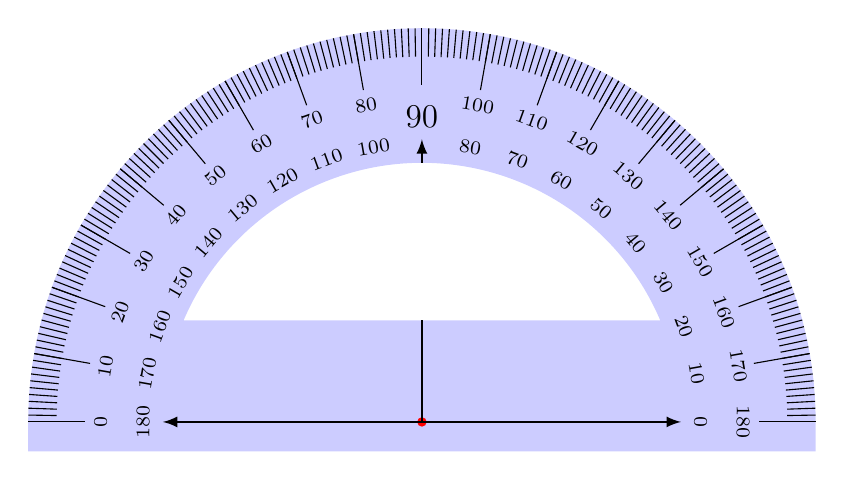
\begin{tikzpicture}
		\pgfmathsetmacro{\radius}{5}
		\pgfmathsetmacro{\innerradius}{\radius*0.658}
		\coordinate(O)at(0,0);
		\coordinate(A0)at(-1,-0.5);
		\coordinate(B0)at(1,-0.5);
		\coordinate(A)at(-1,-0);
		\coordinate(B)at(1,-0);
		% calcul pour la zone intérieure transparente (cap commençant à y=0.3)
		\pgfmathsetmacro{\alpha}{asin(\radius*0.258/\innerradius)} % angle en degrés
		\pgfmathsetmacro{\xcoord}{sqrt(\innerradius*\innerradius - (\radius*0.258)*(\radius*0.258))}
		% remplir en une seule figure : demi-disque supérieur + rectangle sous y=0
		% chemin extérieur : arc de 180° à 0° puis rectangle jusqu'à y=-0.5
		\fill[blue,fill opacity=0.2,even odd rule]
			(O) ++(180:\radius) arc (180:0:\radius) -- ($(O)+(\radius,-0.075*\radius)$) -- ($(O)+(-\radius,-0.075*\radius)$) -- cycle
			% chemin intérieur (cap) à enlever
			({\xcoord},\radius*0.258) -- ({\innerradius*cos(\alpha)},{\innerradius*sin(\alpha)})
			arc (\alpha:180-\alpha:\innerradius) -- ({-\xcoord},\radius*0.258) -- cycle;
		% repère du centre
		\fill[red] (O) circle (0.06);
		% contour du demi-cercle
		% \draw[thick] (O) ++(180:\radius) arc (180:0:\radius);
		% graduations et étiquettes tous les 10° de 0 à 180
		% parcourir 0..80 puis 100..180 pour exclure 90°
		\foreach \innerang in {0,10,...,80,100,110,...,180}{%
			\pgfmathtruncatemacro{\outerangleInt}{180-\innerang}% integer outer angle
			\draw[thin] (O) ++(\innerang:\radius) -- ++(\innerang:-\radius*0.144);
			\node[font=\scriptsize,rotate=\innerang-90] at ($(O)+(\innerang:\innerradius+0.25)$) {\innerang};
			\node[font=\scriptsize,rotate=\innerang-90] at ($(O)+(\innerang:\radius*0.856-0.2)$) {\outerangleInt};
			}
		\draw[thin] (O) ++(90:\radius) -- ++(90:-\radius*0.144);
		\foreach\ang in{0,1,...,180}{%
			\draw[thin] (O) ++(\ang:\radius) -- ++(\ang:-\radius*0.072);
			}
		\draw node at(90:\radius*0.856-0.4){\large 90};
		\draw[thick,-latex] (O) ++(90:\innerradius) -- ++(90:0.3);
		\draw[thick] (O) -- (90:\radius*0.258);
		\draw[thick,latex-latex] (180:\innerradius) -- (0:\innerradius);
	\end{tikzpicture}
\end{document}